\begin{figure}[htbp]
	\centering
	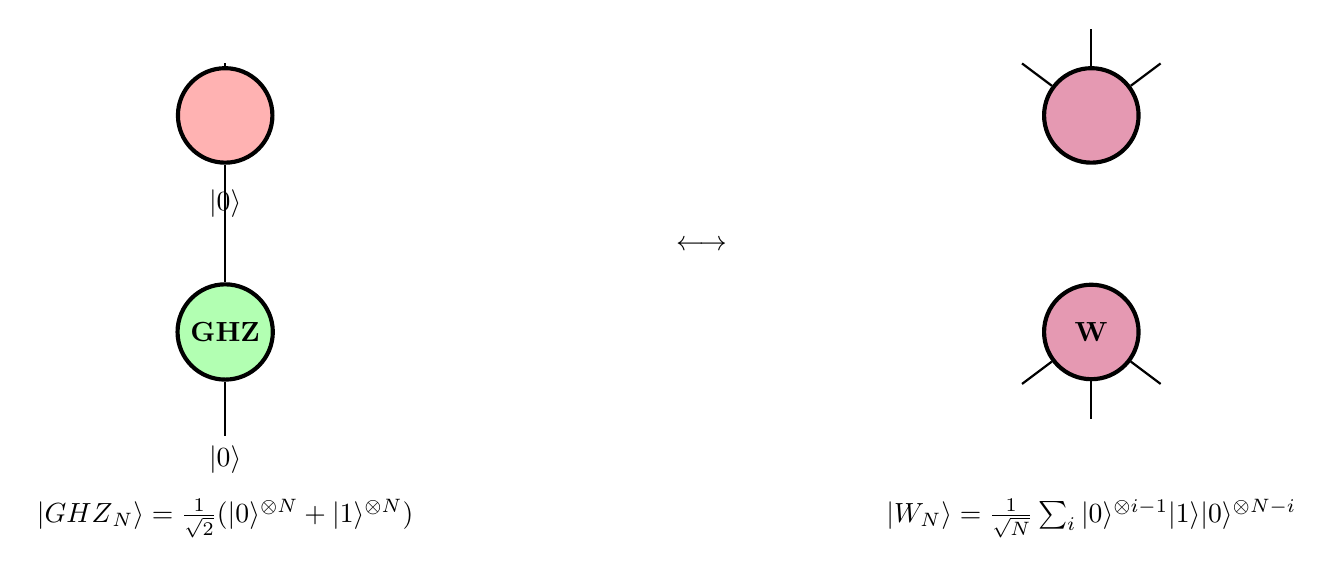
\begin{tikzpicture}[scale=1.1]
		\begin{scope}
			\node[draw, circle, fill=green!30, minimum size=1.2cm, line width=1.5pt] (ghz) at (0,0) {\textbf{GHZ}};
			\draw[thick] (ghz) -- ++(0,1.2) node[above] {$|0\rangle$};
			\draw[thick] (ghz) -- ++(0,-1.2) node[below] {$|0\rangle$};

			\node[draw, circle, fill=red!30, minimum size=1.2cm, line width=1.5pt] (ghz2) at (0,2.5) {};
			\draw[thick] (ghz2) -- ++(0,0.6);
			\draw[thick] (ghz2) -- (ghz);

			\node[below=2.0cm] at (0,0) {$|\text{GHZ}_N\rangle = \frac{1}{\sqrt{2}}(|0\rangle^{\otimes N} + |1\rangle^{\otimes N})$};

		\end{scope}

		\node at (5.5,1) {$\longleftrightarrow$};

		\begin{scope}[xshift=10cm]
			\node[draw, circle, fill=purple!40, minimum size=1.2cm, line width=1.5pt] (w1) at (0,0) {\textbf{W}};
			\node[draw, circle, fill=purple!40, minimum size=1.2cm, line width=1.5pt] (w2) at (0,2.5) {};
			\draw[thick] (w1) -- ++(0,-1);
			\draw[thick] (w2) -- ++(0,1);
			\draw[thick] (w1) -- ++(0.8,-0.6);
			\draw[thick] (w1) -- ++(-0.8,-0.6);
			\draw[thick] (w2) -- ++(0.8,0.6);
			\draw[thick] (w2) -- ++(-0.8,0.6);

			\node[below=2.0cm] at (0,0) {$|W_N\rangle = \frac{1}{\sqrt{N}}\sum_i |0\rangle^{\otimes i-1}|1\rangle|0\rangle^{\otimes N-i}$};

		\end{scope}

	\end{tikzpicture}
	\caption{Comparison of GHZ and W states in ZW calculus notation. GHZ states have maximal entanglement across all bipartitions, while W states have distributed entanglement that survives tracing out any single party. These represent distinct SLOCC equivalence classes for $N \geq 3$.}
	\label{fig:zw-ghz-vs-w}
\end{figure}
